\section{Durchführung}
Zunächst werden die geometrischen Abmessungen der Stäbe mit einem Maßband für die Länge und einer Schiebelehre für die Dicke
gemessen und notiert.
Um die Durchbiegung oder Auslenkung $D(x)$ der Metallstangen zu messen werden diese wie in Abbildung \ref{fig:Messapparatur} gezeigt,
einmal einseitig an Position A und einmal beidseitig an den Positionen A und B eingespannt.
Zwei Messuhren sind an einer geraden Schiene oberhalb der Stange angebracht, um mit der Feder der einen Messuhr das Ergebnis der
anderen Messuhr nicht zu verfälschen, wird jeweils nur eine Messuhr verwendet, die entlang der Stange verschoben wird.
Die nicht verwendete Messuhr wird an der linken auflagepsition des Stabes (vgl Abb.)
Die Messuhren geben eine Auslenkung bis auf \qty{0.001}{\milli\meter} genau an.
Ein Gewicht wird an der Postion $L$ bzw. $L/2$ an der Stange aufgehängt
Weil die Stangen nach langer Benutzung bereits deutlich messbar permanent verformt wurden,
wird bei jedem Messpunkt x die der Abstand ohne Gewicht $(D_0)$ gemessen und anschließend das Gewicht eingehängt 
um den neuen Abstand ($D_m$) zu messen.

\begin{figure} 
    \centering
    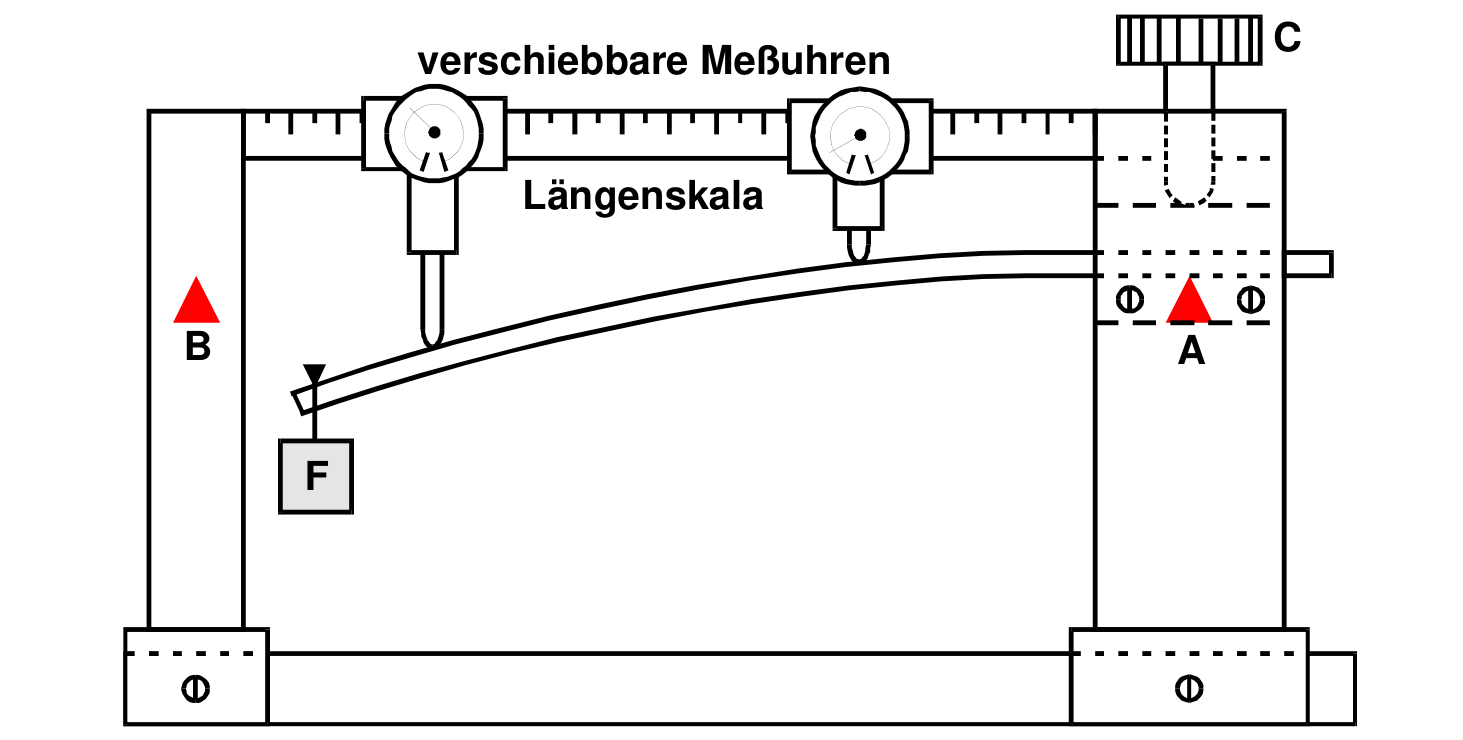
\includegraphics[width=0.8\textwidth]{Abbildungen/Messapperatur.png}
    \caption{Schematische Darstellung der verwendeten Messapparatur.}
    \label{fig:Messapparatur}
\end{figure}